\section{Aufgabe der Komponente}
Über den Broadcast erhält der Benutzer eine Vielzahl an Nachrichten von anderen Benutzern, von denen einen Großteil für ihn irrelevant sind. Der Semantische Filter ist dafür verantwortlich, dem Benutzer nur die für ihn interessante Nachrichten zu akzeptieren und in seine Wissensbasis einfließen zu lassen. Er ist damit neben dem Broadcast die wichtigste Komponente dieser Arbeit. Neben dem bereits beschriebenen Eingangsfilter gibt es noch einen Ausgangsfilter, der für die etwaige Weiterleitung von Nachrichten an andere Peers verantwortlich ist. 
\\Die Benutzer können ihre Filter über ein Menü innerhalb des Profilbereichs einstellen, wobei dies keine Pflicht ist. Wenn keine Filter gesetzt sind, werden alle Nachrichten akzeptiert und weitergeleitet, sofern diese nicht bereits zuvor empfangen worden sind. 

\section{Architektur}

\subsection{Überlick}\label{ch:filtercomps}
Der semantische Filter gliedert sich in verschiedene Teilfilter, diese Trennung richtet sich nach den bereits bekannten Dimensionen des Shark Frameworks. Um den Gesamtfilter mit den kleineren Teilfiltern dynamisch zusammensetzen zu können, wurde das Entwurfsmuster Kompositum gewählt. Mit Hilfe dieses Musters müssen nur jeweils die Teilfilter gesetzt werden, die für den Benutzer auch eine Relevanz haben. Die folgende Klassenhierarchie verdeutlicht dieses Verhältnis:
\begin{figure}[H]
	\centering
	\hspace*{1cm}
	\makebox[\linewidth][c]{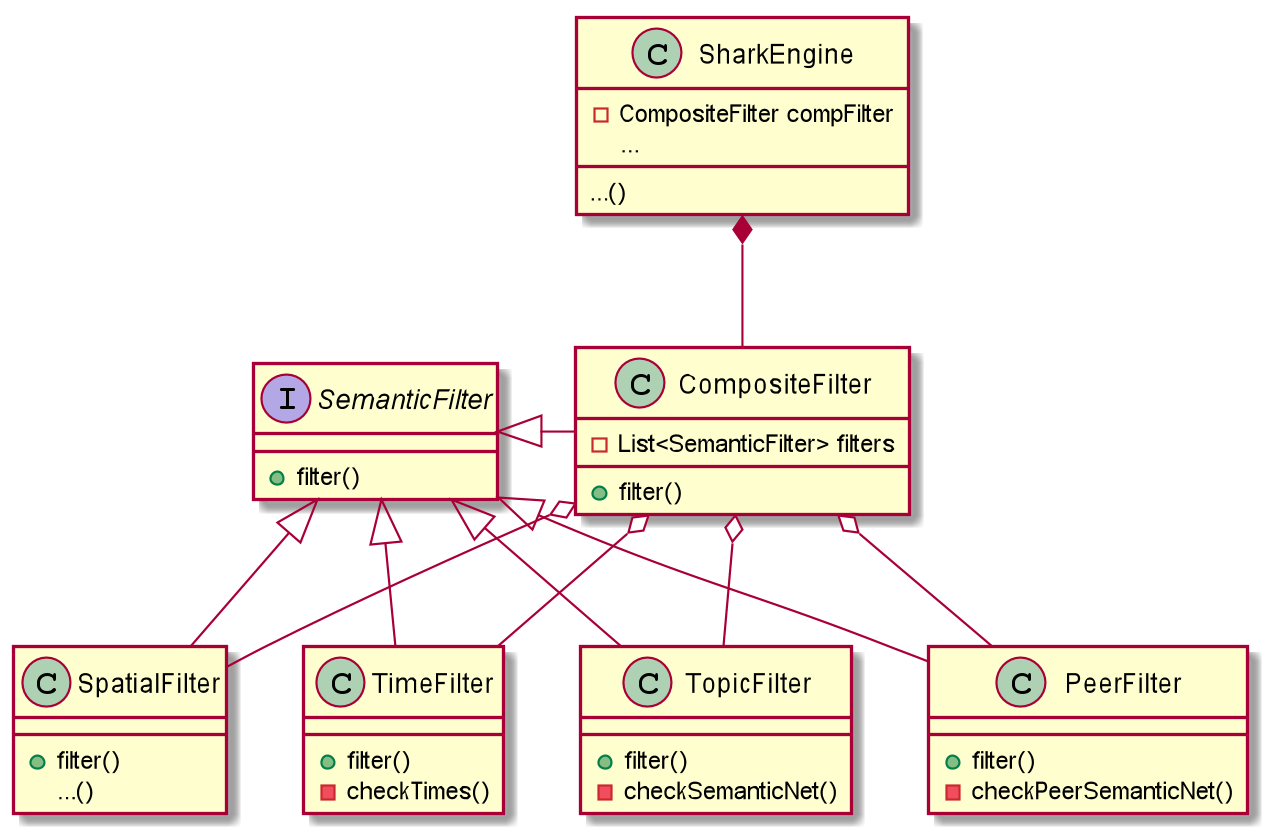
\includegraphics[width=0.9\linewidth]{semanticFilter/images/compositeFilter.png}}%
	\caption{Klassenhierarchie des semantischen Filters (Auszug)}
	\label{fig:broadcastStructure}
\end{figure} 
\begin{itemize}
	\item Die \textit{SharkEngine} enthält das Kompositum und stellt Methoden zur Erzeugung und Anpassung dafür bereit. Weiterhin ist diese Klasse von der App aus erreichbar, wodurch über die App abhangig von den Eingaben des Benutzers die Filter gesetzt oder entfernt werden können.
	\item Das Interface \textit{SemanticFilter} wird von allen Teilfilterklassen und der Kompositumsklasse implementiert. Die einzige zu implementierende Methode ist dabei die Filtermethode, die einen booleschen Wert zurückliefert.
	\item Der \textit{CompositeFilter} besitzt eine Liste aus allen Teilfiltern, ermöglicht durch Polymorphismus. Bei Aufruf der Filtermethode werden sämtliche Teilfilter angewandt, die sich in der Liste befinden. Näheres dazu befindet sich im Unterkapitel 7.3.1 Code. 
	\item Die Relevanz der Themen werden durch den \textit{TopicFilter} geprüft. Der Filter kann für die beiden Dimensionen Topics und Types verwendet werden.
	\item Die Dimensionen Sender, Approvers und Receivers werden durch den PeerFilter abgedeckt. Da die Dimension Sender in Gegensatz zu Approvers und Receivers nur ein SemanticTag, jedoch kein SemanticNet enthält, findet eine Fallunterscheidung am Anfang der Methode statt.
	\item Der \textit{TimeFilter} kontrolliert, ob sich mindestens einer der Zeiträume, die sich im semantischen Profil und in der empfangenen Nachricht befinden, überschneiden. 
	\item Die spatiale Auswertung findet im \textit{SpatialFilter} statt, sie wird im Rahmen einer Bachelorarbeit von Maximilian Öhme entwickelt.
\end{itemize}

\subsection{Code}
Wie bereits im Überblick angerissen, führt der \textit{CompositeFilter} keine eigene semantische Filterung durch, sondern lässt dies fachgerecht von den Teilfiltern ausführen. Im folgenden Codeausschnitt ist erkennbar, dass der sequentielle Aufruf der Teilfilter sofort abgebrochen wird, wenn ein Teilfilter ein \textit{false} liefert.
\lstset{language=Java, caption=Filtermethode im Kompositum, label=DescriptiveLabel, numbers=left, numbersep=1em, breaklines=true, basicstyle=\small}
\begin{lstlisting}
boolean isInteresing = true;
int i = 0;
while (isInteresing && i < childFilters.size()) {
isInteresing =  childFilters.get(i).filter(message, newKnowledge, entryProfile);
i++; }
return isInteresing;
\end{lstlisting}
Angenommen es handelt sich bei der ersten Iteration der Schleife um eine Instanz der Klasse \textit{TopicFilter}, welche ihre Filtermethode aufruft, dann würde es zunächst zur folgenden Auswertung kommen:
\lstset{language=Java, caption=Filtermethode des TopicType Filters (Auszug), label=DescriptiveLabel, numbers=left, numbersep=1em, breaklines=true, basicstyle=\small}
\begin{lstlisting}
if (activeEntryProfile == null) return true;
switch (dimension){
  case TOPIC:
    if (activeEntryProfile.getTopics() instanceof SemanticNet) {
	  isInteresting = checkSemanticNet(activeEntryProfile.getTopics(), newKnowledge);
	}
	else {
	  isInteresting = checkSemanticTag(newKnowledge, activeEntryProfile);
    }
break;
\end{lstlisting}
Es wird zunächst wie auch bei allen anderen Teilfiltern überprüft, ob überhaupt ein semantisches Profil vom Benutzer gesetzt worden ist. Falls nicht, wird die Auswertung sofort mit einem \textit{true} als Rückgabewert beendet. Es wird nun wie auch beim \textit{PeerFilter} Überprüft, um welche Dimension es sich bei der Filterauswertung handelt. In Zeile vier von Listing 7.2 wird überprüft, ob es sich nur um ein einzelnes Tag oder um ein gesamtes SemanticNet handelt. Dadurch wird der Besonderheit in Shark Rechnung getragen, dass eine Dimension entweder durch ein einzelnes Tag oder durch ein komplettes Semantisches Netz beschrieben werden kann. Der folgende Auszug zeigt die Auswertung eines Semantischen Netzes:
\lstset{language=Java, caption=Auswertung des Semantischen Netzes (Auszug), label=DescriptiveLabel, numbers=left, numbersep=1em, breaklines=true, basicstyle=\small}
\begin{lstlisting}
SemanticNet resultNet = SharkCSAlgebra.contextualize(inputNet, profileSet, fp);
	if (resultNet == null || resultNet.isEmpty()) {
		return false;
	}
	else {
		return true;
	}
\end{lstlisting}
Für die Auswertung wird die vom SharkFramework bereitgestellte Funktionalität der Kontextualisierung von Semantischen Netzen benutzt. Die in Zeile dafür aufgerufene Methode benötigt dabei drei Parameter. Diese umfassen das Semantische Netz des Benutzerprofils und das Semantische Netz der Nachricht innerhalb dessen zugeordneten Dimensionen, sowie die Fragmentierungsparameter der Kontextualisierung. 


\subsection{Schnittstellendefinitionen}\label{ch:filterinterfaces}


\section{Nutzung}


\section{Test}



\section{Ausblick}
